\documentclass[tikz,border=10pt]{standalone}
\usepackage{tikz}
\usetikzlibrary{shapes, arrows.meta, positioning, fit, calc}
\usepackage{soul}
\usepackage{textcomp}

% Define styles for nodes
\tikzset{
  level0/.style = {rectangle, draw=black, very thick, minimum width=3cm, minimum height=1cm, text centered, font=\sffamily\bfseries},
  level1/.style = {rectangle, rounded corners, draw=black, very thick, minimum width=2.5cm, minimum height=1cm, text centered, font=\sffamily\bfseries},
  level2/.style = {rectangle, draw=black, thick, minimum width=2.25cm, minimum height=1cm, text centered, font=\sffamily},
  level3/.style = {rectangle, rounded corners, draw=black, thick, font=\ttfamily, text=black, align=center, inner sep=2pt, minimum width=2cm, minimum height = .85cm}
}

\begin{document}
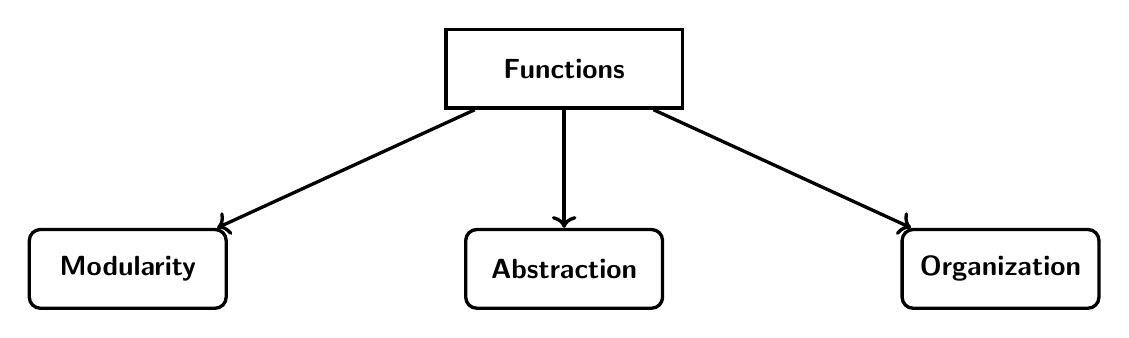
\begin{tikzpicture}
  % Level 0: Functions
  \node (functions) [level0] {Functions};

  % Level 1: Benefits of Functions
  \node (abstraction) [level1, below=1.5cm of functions] {Abstraction};
  \node (modularity) [level1,left = 3 cm of abstraction] {Modularity};
  \node (organization) [level1,  right=3cm of abstraction] {Organization};

  % Connecting Nodes
  \draw[->, very thick, black] (functions) -- (modularity);
  \draw[->, very thick, black] (functions) -- (abstraction);
  \draw[->, very thick, black] (functions) -- (organization);
\end{tikzpicture}
\end{document}
